Using the VI formulation for DTA, we designed a modular and extendable software framework to solve DTA problems. To achieve modularity and expendabilty, we used the object-oriented programming (OOP) method, which employs data abstractions, called \textit{objects}, as the basic structures of software. An object comprise data that is tightly coupled with operations, called \textit{methods}, that can modify it. \textit{Methods} also enable communication among objects. For expendability, we enabled the \textit{inheritance} concept in OOP, which is the capability of new objects to build on properties (data and methods) of existing objects. Inheritance allows the creation of new objects that build on existing objects to extend the original objects\cite{ten1989object}.

\begin{figure}[h]
    \centering
    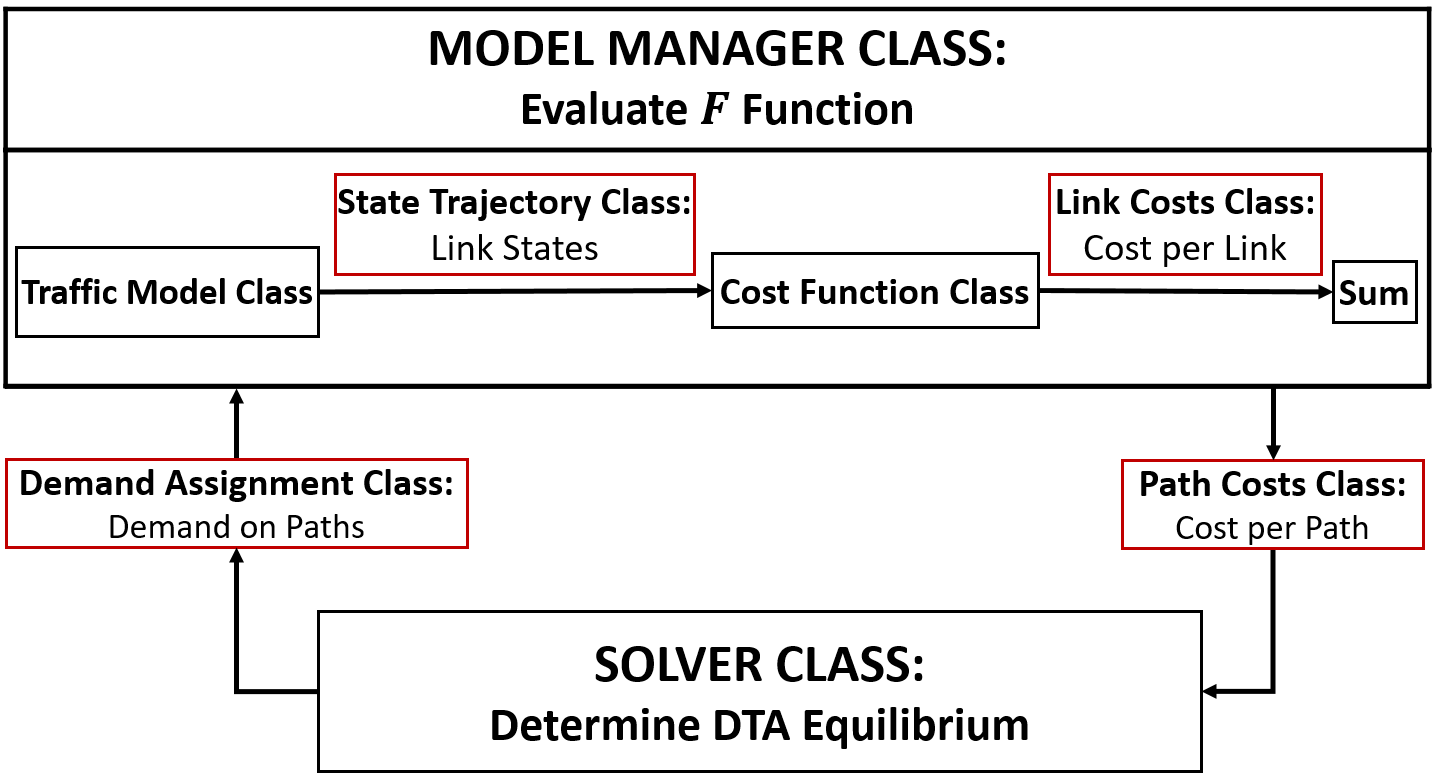
\includegraphics[width=\linewidth]{Class_Diagram.PNG}
    \caption{Software Framework Architecture}
    \label{fig:class_diagram}
\end{figure}

To describe the software structure, we use a class diagram shown in  Figure~\ref{fig:class_diagram}. A class diagram represents an object in OOP software using the class template. Class diagrams are one the main modeling tools for OOP software. As shown in Figure~\ref{fig:class_diagram}, our software framework architecture follows closely the VI formulation. It has two main classes: the Model Manager class, which implements the $F$ function, and the Solver class, which implements algorithms that determine the DTA equilibrium. 

The Model Manager class implements the $F$ function, which translates demands on paths (an assignment) to the corresponding path costs. Assignments are implemented by the Demand Assignment class, while path costs are represented by the Path Costs class. Figure~\ref{fig:class_diagram} also show that the Model Manager class is further divided into three main classes that correspond to the $F = \Sigma\circ c \circ \mathbb{T}$ composition function previously defined. The Traffic Model class is the $\mathbb{T}$ and converts demands on paths to demands on links to get link states, which are represented by the State Trajectory class. The Cost Function class  ($c$ operation) translates the link states to link costs, represented by the Link Costs class. The $\Sigma$ operator is implemented by the Sum module that adds the link costs for each path and outputs the costs per path. 

The Solver class calls 

The advantage of our modular software framework is that it can be easily extended by building on existing traffic model, cost function, and solver classes. We developed the traffic model, cost function, and solve classes as basic building blocks for actual traffic models, cost functions, and solver algorithms that a user might want to implement.Users can expand on them using the inheritance concept in OOP. For example, the software framework currently include three traffic models: the static model, Merchant and Nemhauser (MN) model, and the Point Queue Model, which are all extensions of the basic traffic model class. It also has a cost function based on travel time, that can be replaced by an energy or emission based cost function. We included three solver algorithms: the Method of Successive Averages, the Frank-Wofle Algorithm, and the Extra Projection Methods, which are applied depending on the $F$ function properties. The demand assignment, state trajectory, link costs, and path costs classes provide the format for the input/output messages among the other modules, and are not extendable.  

Given an assignment $h'$, a DTA solution algorithm needs the cost for each path, $F_p(h^')$ $\forall p\in\mathcal{P}$, to determine if $h'$ is an equilibrium assignment according to equation (x). Accordingly, a DTA solution algorithm implemented in the framework will use the Model Manager module via Solver interface to translate assignments to their corresponding path costs $F(h)$. The path costs allow the algorithm to determine whether it has reached equilibrium or whether/how it needs to adjust its current assignment to move towards the equilibrium state.

\item Ziliaskopoulos and Waller developed VISTA,
an internet-based geographic information system that integrates transportation spatio-temporal data and models into a single framework. While VISTA does integrate analytical and simulation-based DTA models along with DTA solution algorithms, it was built with particular focus on the integration of different transportation modules. This is unlike \textit{ta\_solver} that was designed to solve DTA problems. In addition, VISTA has no fundamental DTA problem formulation, while \textit{ta\_solver} is based on VI. 

Currently
Contributions:
\begin{enumerate}
\item A clear and unified variational inequality formulation for traffic assignment problems (with good notation).
\item A modular software framework, \textit{ta\_solver},  with solvers based on the unified variational inequality formulation.
\item Demonstration of the performance of the software framework using different models.
\end{enumerate}